\chapter{Arquitectura del sistema y lógica del código (backend en Go)}

\section{Filosofía de diseño}

El proyecto se organiza en cuatro capas desacopladas. La Figura~\ref{fig:arquitectura} resume la arquitectura; el paquete \texttt{scapegoat} no importa \texttt{database}, \texttt{net/http} ni persistencia, lo que permite ejecutar \texttt{go test ./scapegoat/...} de forma aislada.

\begin{figure}[H]
  \centering
  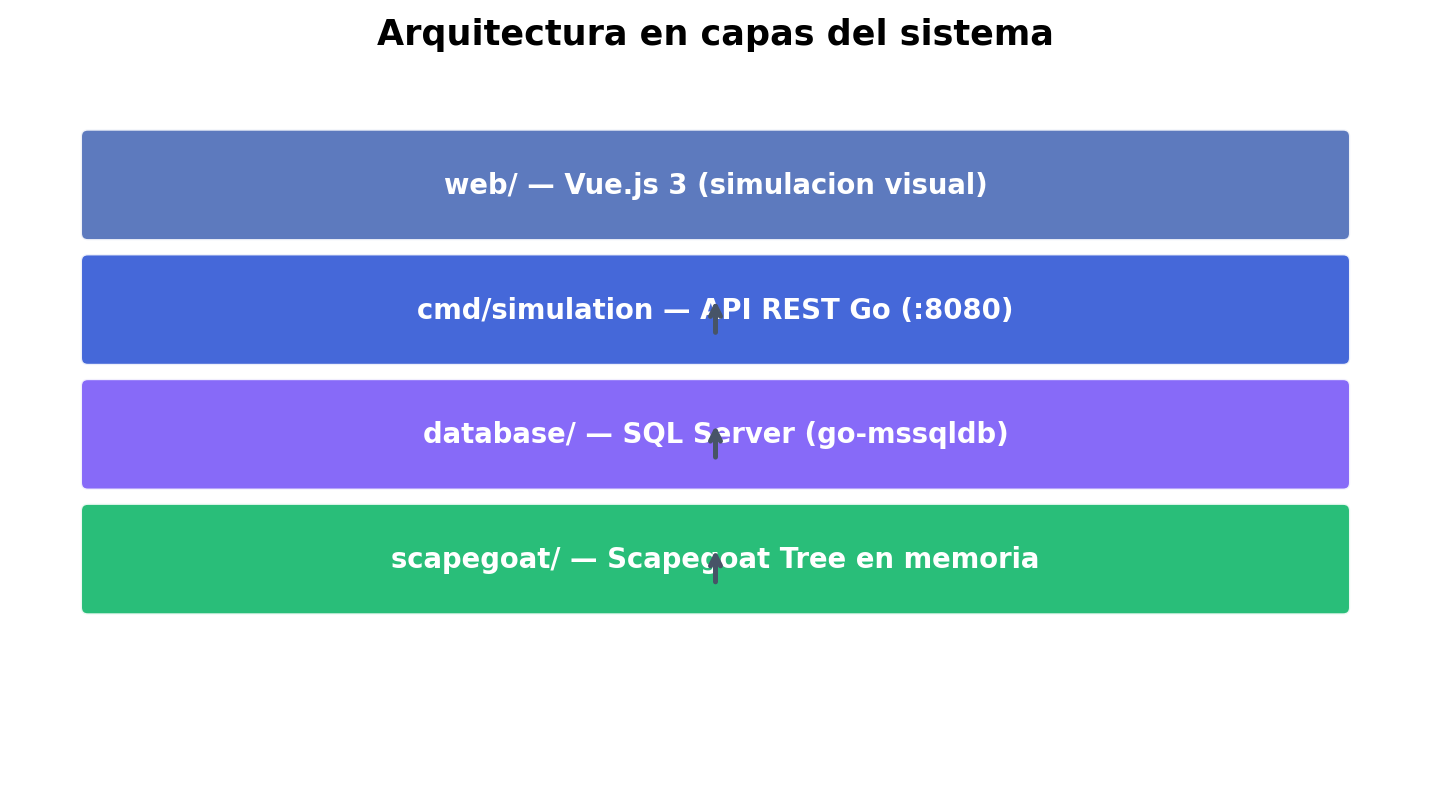
\includegraphics[width=0.88\textwidth]{diagrams/01-arquitectura.png}
  \caption{Arquitectura en capas del sistema}
  \label{fig:arquitectura}
\end{figure}

Go 1.18+ habilita \textbf{genéricos}. Usamos \go{Tree[K, V any]} con comparador externo, \go{NewOrdered[K Ordered, V any]} para tipos ordenados, y punteros \go{*node[K,V]} para hijos izquierdo y derecho.

\section{Tipos y estructuras de datos}

\subsection{Nodo interno}

\begin{lstlisting}[style=gocode,caption={Estructura de nodo interno},label={lst:node}]
type node[K, V any] struct {
    key         K
    value       V
    left, right *node[K, V]
}
\end{lstlisting}

\subsection{Árbol público}

\begin{lstlisting}[style=gocode,caption={Estructura Tree con contadores n, q y alpha},label={lst:tree}]
type Tree[K, V any] struct {
    root         *node[K, V]
    less         func(K, K) bool
    alpha        float64
    n, q         int
    rebuilds     int
    rebuiltNodes int
}
\end{lstlisting}

\begin{table}[H]
  \centering
  \caption{Campos de la estructura \texttt{Tree}}
  \begin{tabular}{@{}lp{9cm}@{}}
    \toprule
    \textbf{Campo} & \textbf{Rol} \\
    \midrule
    \texttt{root} & Puntero a la raíz; \texttt{nil} si el árbol está vacío \\
    \texttt{less} & Relación de orden estricto: \texttt{less(a,b)} $\Leftrightarrow$ $a < b$ \\
    \texttt{alpha} & Parámetro de balance $\alpha \in (0.5, 1)$ \\
    \texttt{n}, \texttt{q} & Contadores de nodos actuales y máximo desde última rebuild global \\
    \texttt{rebuilds} & Número de reconstrucciones realizadas \\
    \bottomrule
  \end{tabular}
\end{table}

\section{Catálogo de funciones principales}

\subsection{Constructores}

\go{New[K,V](alpha, less)} valida $\alpha \in (0.5, 1)$ y que \texttt{less} no sea \texttt{nil}. \texttt{NewOrdered} inyecta \go{less = func(a,b) bool { return a < b }}.

\subsection{Búsqueda e inserción}

\texttt{Search(key)} realiza búsqueda BST iterativa en $\bigO(h)$ donde $h$ es la altura. \texttt{Insert} y \texttt{InsertWithTrace} delegan en \texttt{insert}, que:
\begin{enumerate}[noitemsep]
  \item Inserta como BST ordinario.
  \item Incrementa $n$ y $q$ si la clave es nueva.
  \item Si $\mathrm{depth} > d_{\max}(q)$, asciende el camino buscando el scapegoat (Ec.~\ref{eq:scapegoat-cond}).
  \item Reconstruye el subárbol con \texttt{flatten} + \texttt{buildBalanced}.
\end{enumerate}

\subsection{Eliminación}

\texttt{Delete(key)} aplica eliminación BST clásica (tres casos). Si $n < \alpha \cdot q$, ejecuta reconstrucción global (Ec.~\ref{eq:global-rebuild}).

\subsection{Detección del scapegoat}

\begin{lstlisting}[style=gocode,caption={Fragmento de detección de scapegoat en inserción},label={lst:scapegoat}]
if depth > t.maxDepth(t.q) {
    for i := len(path) - 2; i >= 0; i-- {
        parent, child := path[i], path[i+1]
        if float64(size(child)) > t.alpha*float64(size(parent)) {
            scapegoatKey := parent.key
            trace.Scapegoat = &scapegoatKey
            flattenKeys(parent, &trace.RebuiltKeys)
            rebuilt := t.rebuild(parent)
            // Reenlazar rebuilt en el arbol...
            break
        }
    }
}
\end{lstlisting}

\subsection{Reconstrucción balanceada}

\begin{equation}
  d_{\max} = \left\lfloor \frac{\ln q}{\ln (1/\alpha)} \right\rfloor
\end{equation}

\texttt{rebuild(root)} aplana el subárbol in-order, incrementa contadores y llama \texttt{buildBalanced}, que selecciona el nodo medio garantizando altura $\lfloor \log_2 k \rfloor$ para $k$ nodos.

\begin{figure}[H]
  \centering
  \begin{tikzpicture}[
    box/.style={rectangle, draw, rounded corners, minimum width=2.2cm, minimum height=0.8cm, align=center, font=\small},
    arrow/.style={-{Stealth[length=2mm]}, thick}
  ]
    \node[box, fill=red!8] (a) {Subárbol desbalanceado};
    \node[box, fill=yellow!12, right=1.6cm of a] (b) {flatten in-order};
    \node[box, fill=yellow!12, right=1.2cm of b] (c) {buildBalanced};
    \node[box, fill=green!10, right=1.6cm of c] (d) {Subárbol balanceado};
    \draw[arrow] (a) -- (b);
    \draw[arrow] (b) -- (c);
    \draw[arrow] (c) -- (d);
  \end{tikzpicture}
  \caption{Proceso de reconstrucción (\texttt{rebuild})}
  \label{fig:rebuild}
\end{figure}

\section{Desafíos técnicos}

El cálculo de \texttt{size(u)} sin campo almacenado eleva el costo de detección. Con $n=1000$ e inserciones ordenadas observamos 375 reconstrucciones y 9762 nodos reconstruidos acumulados. La concurrencia se resuelve con \texttt{sync.Mutex} en la capa HTTP, no dentro del paquete \texttt{scapegoat}.
